\makeatletter\@specialfalse\makeatother
%%%%%%%%%%%%%%%%%%%%%%%%%%%%%%%%%%%%%%%%%%%
%%%%%%  STYLE 01
%%%%%%%%%%%%%%%%%%%%%%%%%%%%%%%%%%%%%%%%%%%


\cxset{
 name={},
 numbering=arabic,
 number font-size=\LARGE,
 number font-family=\rmfamily,
 number font-weight=\bfseries,
 number before=,
 number dot=,
 number after=,
 number position=leftname,
 chapter font-family=\sffamily,
 chapter font-weight=\normalfont,
 chapter font-size=\Large,
 chapter before={\vspace*{20pt}\par},
 chapter after={\hfill\hfill\par},
 chapter color={black!90},
 number color=\color{purple},
 title beforeskip={\vspace*{30pt}},
 title afterskip={\vspace*{40pt}\par},
 title before={},
 title after={},
 title font-family=\sffamily,
 title font-color=\color{purple},
 title font-weight=\bfseries,
 title font-size=\LARGE,
 header style=headings}

\cxset{headings ruled-01}

\chapter{Introduction to Style One}


\begin{summary}
This design is simple and its distinguishing characteristic is a short summary at the beginning of the chapter. This is almost like an abstract typeset in italic font without setting the margins in. We provide a \lstinline{summary} environment for convenience. Note the very simple line in the running head to the left of the page number.
\end{summary}

\medskip
\begin{figure}[ht]
\centering
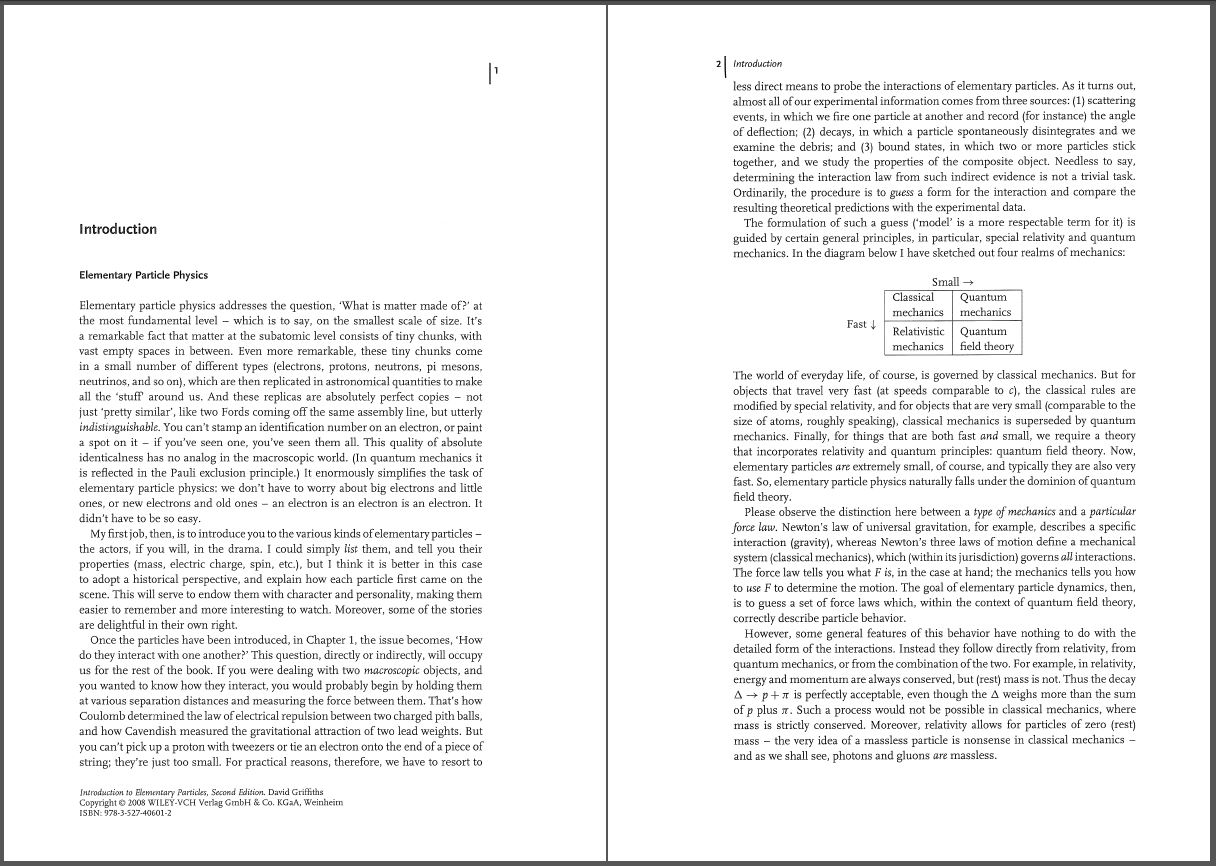
\includegraphics[width=0.5\textwidth]{./chapters/chapter01}
\end{figure}

